\documentclass[border=15pt]{standalone}
\usepackage{amsmath,amssymb,mathtools,bm}
\usepackage{tikz}
\usepackage{pgfplots}
\usepackage{pgf}
\begin{document}
	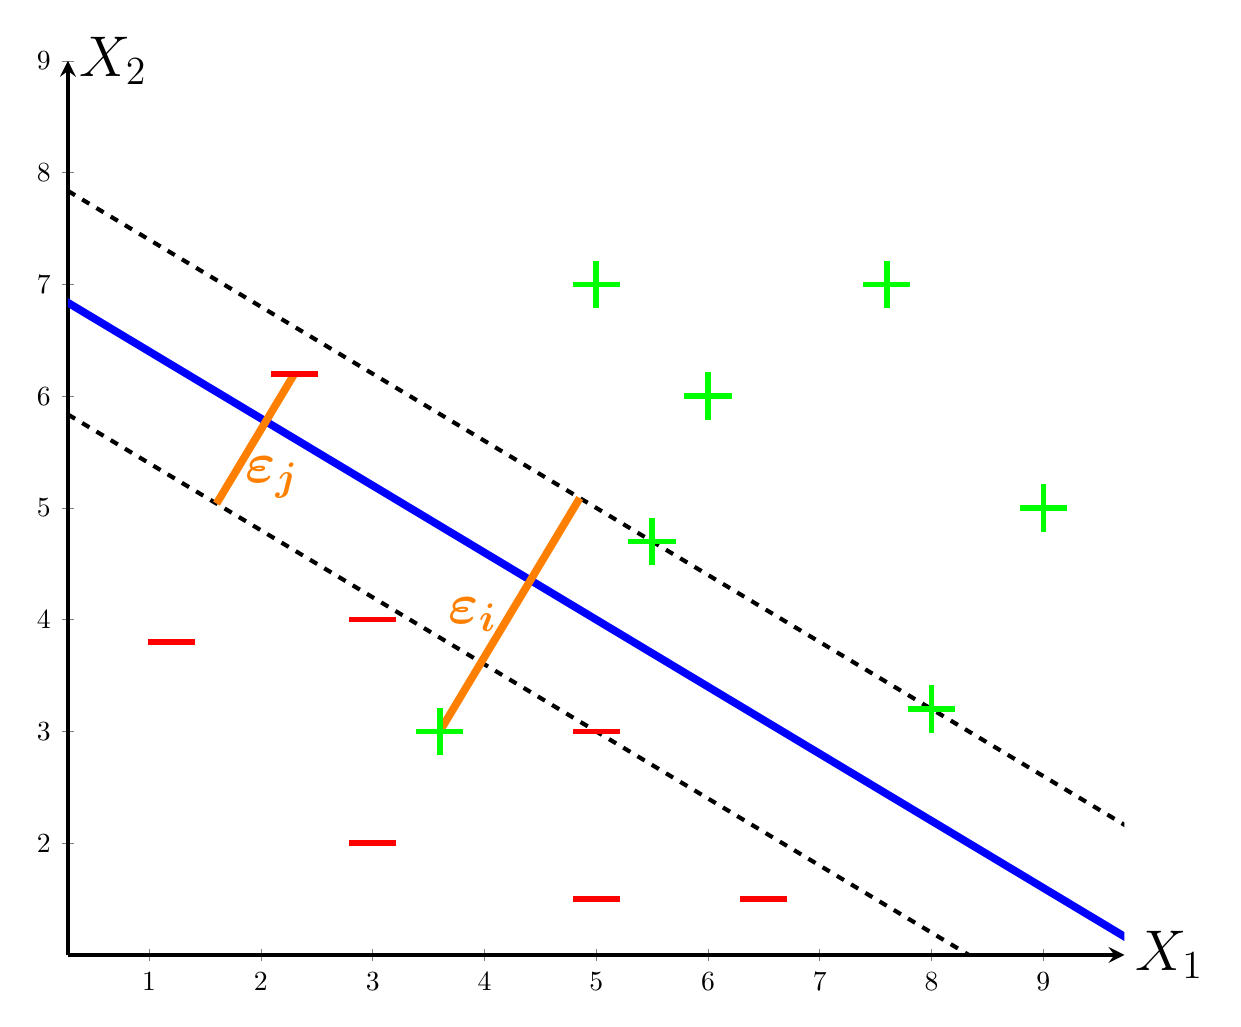
\begin{tikzpicture}
		\begin{axis}[
			xmin=1,
			xmax=9,
			ymin=1,
			ymax=9,
			axis equal,
			width=15cm,
			axis x line=center,
			axis y line=center,
			%xmajorticks=false,
			%ymajorticks=false,
			ylabel style={right,font=\huge},
			ylabel=$X_2$,
			xlabel style={above,right,font=\huge},
			xlabel=$X_1$,
			line width=1.5pt
			]
			%\addplot[no markers, domain=-1:11]{(5/3)*x};
			
		\addplot[only marks, mark=+,draw=green,mark size=0.3cm,line width= 2pt]coordinates {(8,3.2)
			(8,3.2) (5,7) (6,6) (9,5) (7.6,7) (5.5,4.7) (3.6,3)};
		\addplot[only marks, mark=-,draw=red,mark size=0.3cm,line width=2pt]coordinates {(3,4)
			(5,3) (3,2) (5,1.5) (4,0.5) (6.5,1.5) (1.2,3.8) (2.3,6.2)};
			\addplot[no markers,domain=-1:11,thick,blue,line width=2.8pt]{-0.6*x+7};
			\addplot[no markers, domain=-1:11,dashed,line width=1.5pt]{-0.6*x+8};
			\addplot[no markers, domain=-1:11,dashed,line width=1.5pt]{-0.6*x+6};
			\draw[black,thick,orange,line width=2.8pt] (axis cs:2.3,6.2)--(axis cs:1.603,5.0382)node[right,pos=0.8,font=\huge]{$\bm{\varepsilon_j}$};
			\draw[black,thick,orange,line width=2.8pt] (axis cs:3.6,3)--(axis cs:4.853,5.0882) node[left,pos=0.5,font=\huge]{$\bm{\varepsilon_i}$};
		\end{axis}
	\end{tikzpicture}
\end{document}